\documentclass[12pt, a4paper]{article}
% --- Packages ---
\usepackage[utf8]{inputenc}
\usepackage[T1]{fontenc}
\usepackage[french]{babel}
\usepackage{graphicx} % Make sure this is here for images
\usepackage{booktabs}
\usepackage{amsmath}
\usepackage{geometry}
\usepackage{array}
\usepackage{enumitem}
\usepackage{hyperref}
\usepackage{xcolor}
\usepackage{titlesec}
\usepackage{lmodern}
\usepackage{microtype}
\usepackage{fancyhdr}
% --- Font Configuration ---
% --- Color Definitions ---
\definecolor{primary}{RGB}{0,51,102}
\definecolor{secondary}{RGB}{102,102,153}
\definecolor{accent}{RGB}{204,0,0}
% --- Page Geometry ---
\geometry{
  a4paper,
  left=2.5cm,
  right=2.5cm,
  top=2.5cm,
  bottom=2.5cm,
  headheight=15pt
}
% --- Header/Footer Setup ---
\pagestyle{fancy}
\fancyhf{}
\fancyhead[L]{\small Rapport de Stage - Semaine 2}
\fancyhead[R]{\small Zakaria el Khaldi}
\fancyfoot[C]{\thepage}
\renewcommand{\headrulewidth}{0.4pt}
\renewcommand{\footrulewidth}{0.4pt}
% --- Title Formatting ---
\titleformat{\section}
  {\normalfont\Large\bfseries\color{primary}}
  {\thesection}{1em}{}
\titleformat{\subsection}
  {\normalfont\large\bfseries\color{secondary}}
  {\thesubsection}{1em}{}
\titleformat{\subsubsection}
  {\normalfont\normalsize\bfseries\color{accent}}
  {\thesubsubsection}{1em}{}
% --- List Formatting ---
\setlist[itemize]{leftmargin=*, nosep}
\setlist[enumerate]{leftmargin=*, nosep}
% --- Hyperlink Setup ---
\hypersetup{
  colorlinks=true,
  linkcolor=primary,
  urlcolor=secondary,
  citecolor=accent
}
% --- Title Page Information ---
\title{\Huge\bfseries\color{primary} Rapport de Stage \\ 
      \Large Semaine 2 : Développement de l'Interface Utilisateur de la Plateforme E-learning}
\author{\Large Zakaria el Khaldi}
\date{\large Le 17 mai 2025}
% --- Document Start ---
\begin{document}
% --- Cover Page ---
\begin{titlepage}
  \centering
  \vspace*{\stretch{0.5}}
  {\Huge\bfseries\color{primary} Rapport de Stage \par}
  \vspace{1cm}
  {\Large\itshape Semaine 2 : Développement de l'Interface Utilisateur de la Plateforme E-learning\par}
  \vspace{2cm}
  
  \vspace{2cm}
  {\Large Zakaria el Khaldi\par}
  \vfill
  {\large Le 13 mai 2025\par}
  \vspace*{\stretch{1}}
\end{titlepage}
% --- Table of Contents ---
\tableofcontents
\thispagestyle{empty}
\newpage
% --- Introduction ---
\section{Introduction}
\thispagestyle{fancy}
Ce rapport détaille les travaux réalisés durant la deuxième semaine de stage. Suite à la première semaine consacrée à la conception et à l'architecture de la plateforme, cette deuxième semaine a été principalement dédiée au développement frontend avec Next.js. L'objectif principal était de créer la structure du projet, mettre en place les routes et développer l'interface de la page d'accueil.

% --- Week 2 Accomplishments ---
\section{Bilan de la Semaine 2}

\subsection{Mise en place du projet Next.js}

Durant cette semaine, j'ai démarré le développement du frontend de la plateforme e-learning "LearnExpert" en utilisant Next.js. La première étape a consisté à configurer l'environnement de développement et à structurer le projet. Voici les principales tâches accomplies :

\begin{itemize}
  \item Installation et configuration de Next.js avec TypeScript
  \item Mise en place de l'architecture du projet selon les bonnes pratiques
  \item Configuration des outils de développement (ESLint, Prettier)
  \item Installation des dépendances nécessaires (TailwindCSS, React Icons, etc.)
\end{itemize}

\subsection{Création des pages et mise en place des routes}

Une fois le projet configuré, j'ai travaillé sur la création des différentes pages et la mise en place du système de routage :

\begin{itemize}
  \item Création des pages principales (accueil, fonctionnalités, tarification, FAQ, contact)
  \item Implémentation du système de routage avec le routeur intégré de Next.js
  \item Création des composants réutilisables pour la navigation
  \item Mise en place des redirections et gestion des erreurs 404
\end{itemize}

\subsection{Développement de la page d'accueil}

La majeure partie de mon temps a été consacrée au développement de la page d'accueil, qui est désormais complétée à environ 80\%. Voici les éléments développés :

\begin{itemize}
  \item En-tête avec navigation et boutons d'action (Connexion, Inscription)
  \item Section héro avec titre accrocheur et description de la plateforme
  \item Section de présentation des fonctionnalités principales
  \item Section des parcours d'apprentissage et technologies disponibles
  \item Témoignages d'utilisateurs
  \item Section d'appel à l'action
  \item Pied de page avec liens importants et formulaire d'abonnement
\end{itemize}

\subsection{Conception des composants UI réutilisables}

Pour faciliter le développement et maintenir une cohérence visuelle sur l'ensemble de la plateforme, j'ai créé plusieurs composants UI réutilisables :

\begin{itemize}
  \item Composants de navigation (Navbar, Footer)
  \item Boutons de différents styles et tailles
  \item Cartes pour présenter les cours et fonctionnalités
  \item Badges et étiquettes
  \item Composants de formulaire (champs de texte, listes déroulantes, etc.)
\end{itemize}

\section{Progression du projet}

\subsection{État d'avancement}

À l'issue de cette deuxième semaine, le développement frontend progresse comme prévu :

\begin{itemize}
  \item Structure du projet Next.js : 100\% terminée
  \item Système de routage : 100\% terminé
  \item Page d'accueil : 80\% terminée
  \item Composants UI réutilisables : 10\% terminés
  \item Pages secondaires : 20\% terminées (par exemple, FAQ, Contact, Tarification en tant que pages dédiées)
\end{itemize}

\subsection{Captures d'écran des réalisations}

Les images ci-dessous illustrent l'état actuel du développement de l'interface utilisateur de la page d'accueil.
\textit{(Assurez-vous que les noms de fichiers des images ci-dessous correspondent à ceux que vous avez téléversés, par exemple \texttt{home\_hero\_accelerate.png}, \texttt{learning\_journey\_section.png}, \texttt{pricing\_section.png}, etc. Ajustez les noms et les largeurs si nécessaire.)}

\begin{figure}[h!]
  \centering
  
\includegraphics[width=0.9\textwidth]{herosection.png} 
  % This corresponds to the image with "Accelerate Your Tech Career..."
  \caption{Page d'accueil - Section Héro Principale}
  \label{fig:home_hero_accelerate}
\end{figure}

\begin{figure}[h!]
  \centering
  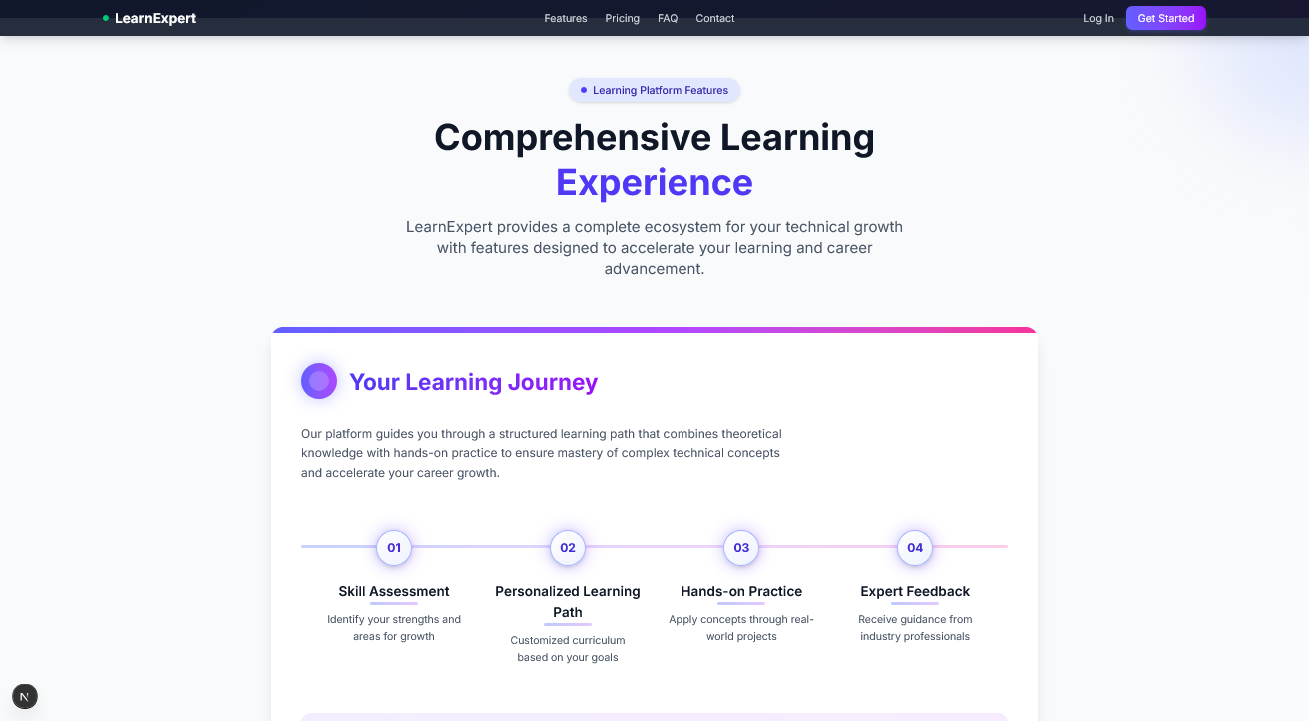
\includegraphics[width=0.9\textwidth]{featchersection_1.png} 
  % This corresponds to the image with "Comprehensive Learning Experience" and "Your Learning Journey"
  \caption{Page d'accueil - Section Parcours d'Apprentissage}
  \label{fig:learning_journey}
\end{figure}

\begin{figure}[h!]
  \centering
  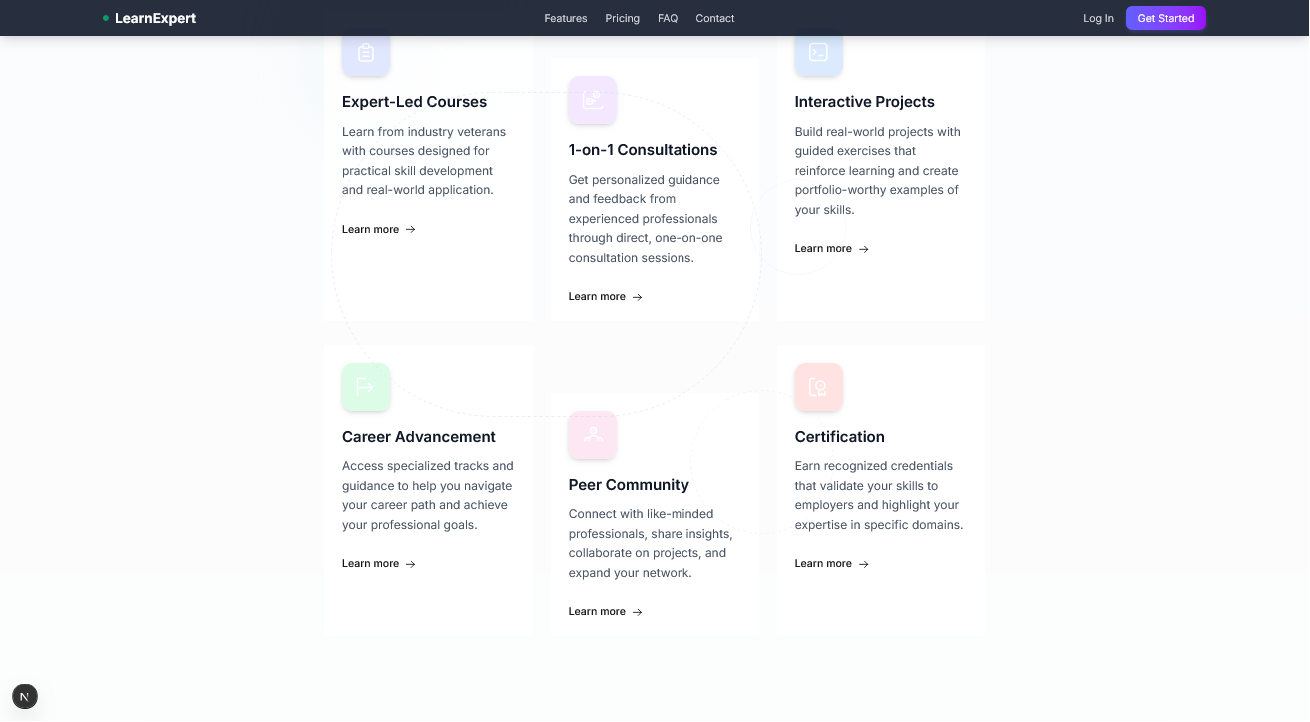
\includegraphics[width=0.9\textwidth]{fetchersection_2.png} 
  % This corresponds to the grid of 6 features: Expert-Led Courses, 1-on-1 Consultations, etc.
  \caption{Page d'accueil - Aperçu des Fonctionnalités}
  \label{fig:features_overview_grid}
\end{figure}

\begin{figure}[h!]
  \centering
  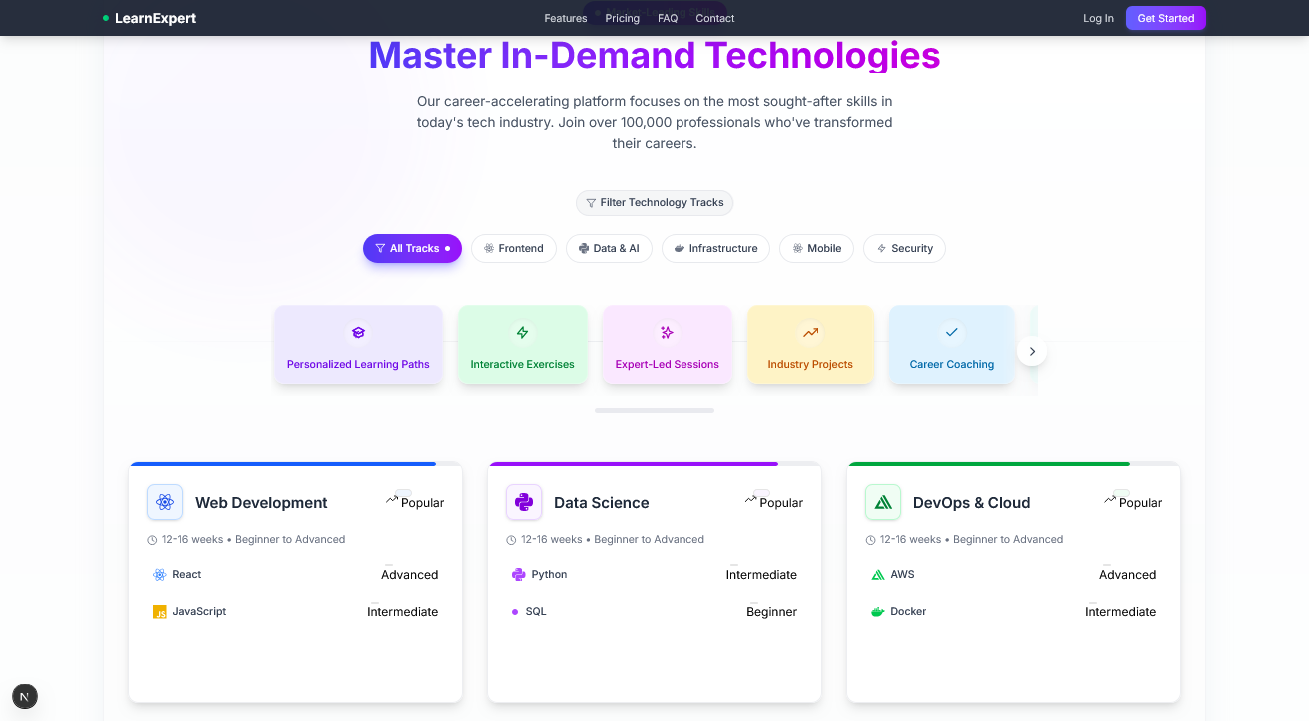
\includegraphics[width=0.9\textwidth]{fetchersection_3.png} 
  % This corresponds to "Master In-Demand Technologies"
  \caption{Page d'accueil - Section des Technologies}
  \label{fig:technologies}
\end{figure}

\begin{figure}[h!]
  \centering
  
\includegraphics[width=0.9\textwidth]{second_call_of_action.png} 
  % This corresponds to "Choose the Perfect Plan for Your Goals"
  \caption{Page d'accueil - Section de Tarification (aperçu)}
  \label{fig:pricing_section}
\end{figure}

\begin{figure}[h!]
  \centering
  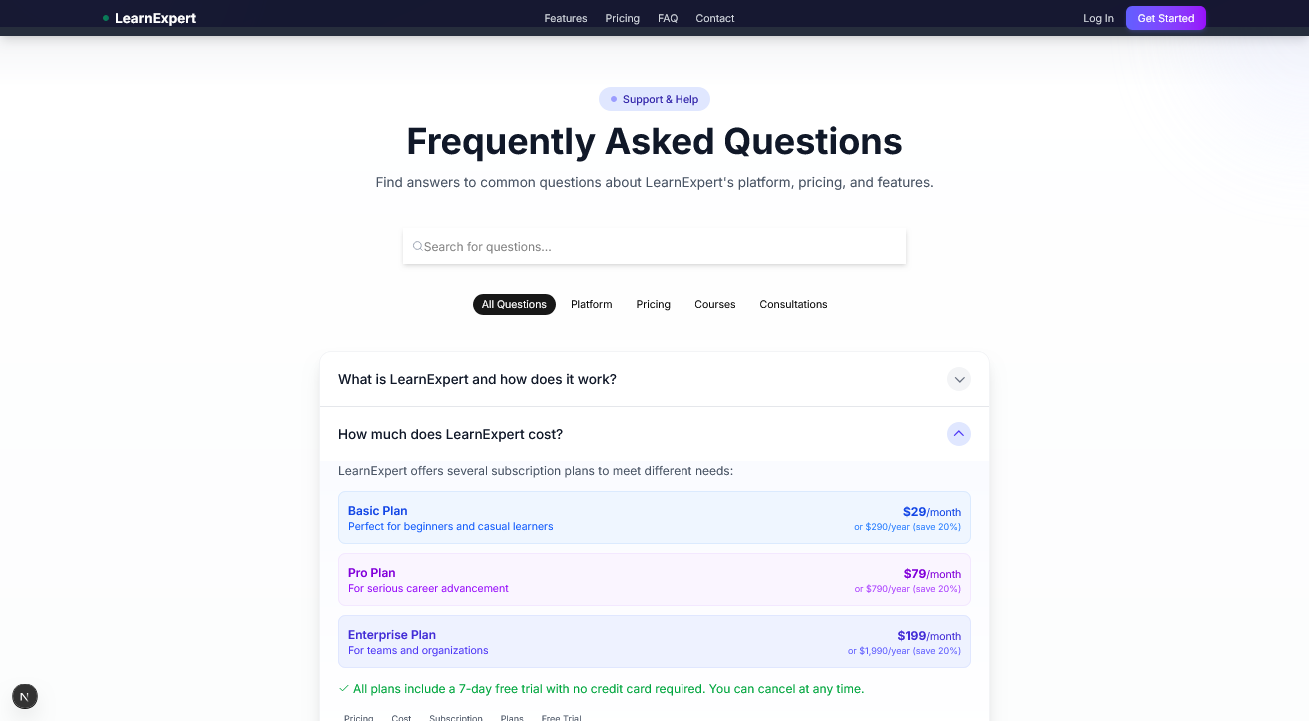
\includegraphics[width=0.9\textwidth]{faqsection.png} 
  % This corresponds to the "Frequently Asked Questions" page view
  \caption{Page des Questions Fréquemment Posées (FAQ)}
  \label{fig:faq_page}
\end{figure}

\begin{figure}[h!]
  \centering
  \includegraphics[width=0.9\textwidth]{contectus.png} 
  % This corresponds to the "We're here to help" contact page view
  \caption{Page de Contact}
  \label{fig:contact_page}
\end{figure}

\begin{figure}[h!]
  \centering
  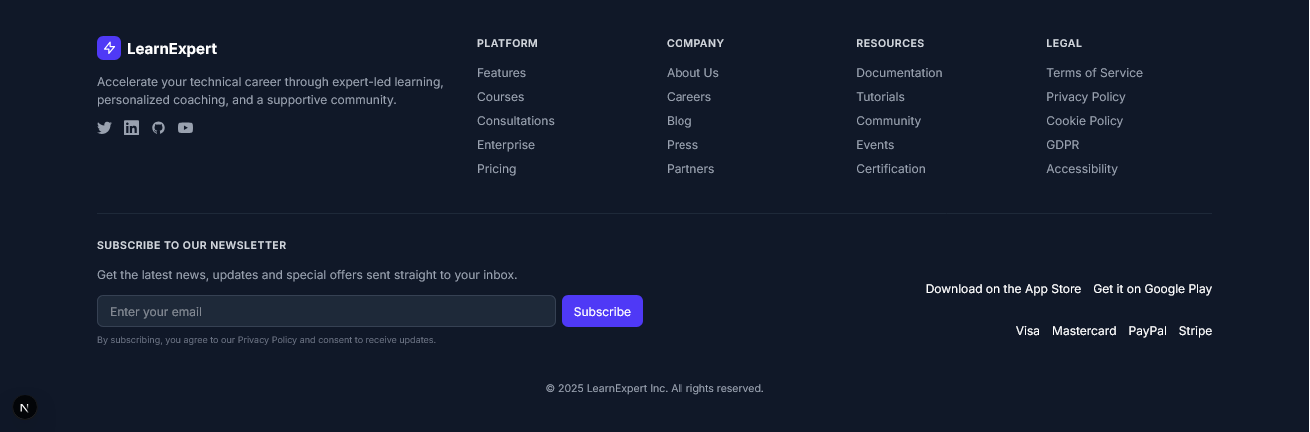
\includegraphics[width=0.9\textwidth]{foter.png} 
  % This corresponds to the main footer section
  \caption{Pied de page principal du site}
  \label{fig:footer_main}
\end{figure}

% Clear the page if figures are taking up too much space before next section
\clearpage 

\section{Difficultés rencontrées et solutions}

Pendant cette semaine de développement, j'ai fait face à quelques défis techniques :

\begin{itemize}
  \item \textbf{Responsive design} : Assurer que l'interface s'adapte parfaitement à tous les appareils a nécessité des ajustements minutieux avec TailwindCSS.
  \item \textbf{Optimisation des performances} : Pour garantir des temps de chargement rapides, j'ai implémenté le chargement différé des images et l'optimisation automatique avec Next.js Image.
  \item \textbf{Cohérence des styles} : La création d'un système de design cohérent a nécessité la mise en place d'un thème centralisé avec des variables CSS personnalisées via TailwindCSS theme configuration.
\end{itemize}

\section{Prochaines étapes}

Pour la semaine à venir, je prévois de :

\begin{itemize}
  \item Finaliser la page d'accueil et corriger les éventuels problèmes d'affichage sur différents navigateurs et appareils.
  \item Terminer le développement des pages secondaires (ex: page de détails d'un cours si non commencée).
  \item Commencer le développement de l'interface utilisateur principale de l'application (tableau de bord apprenant).
  \item Créer les composants nécessaires pour le tableau de bord de l'apprenant.

\end{itemize}

\section{Conclusion}

Cette deuxième semaine a été productive et a permis de réaliser des avancées significatives dans le développement frontend de la plateforme LearnExpert. La structure du projet est désormais en place, et la majeure partie de l'interface de la page d'accueil et des pages d'information clés est développée.

Le travail effectué cette semaine pose des bases solides pour la suite du développement, notamment pour l'interface principale de l'application qui sera au cœur de l'expérience utilisateur de la plateforme e-learning.

\end{document}